\chapter{Time Series Classification Architectures}
\label{ch:series-architectures}

Where uncited, model architectures were generated using the \verb|visualkeras| library\cite{Gavrikov2020VisualKeras}.

\begin{figure}[h]
    \centering
    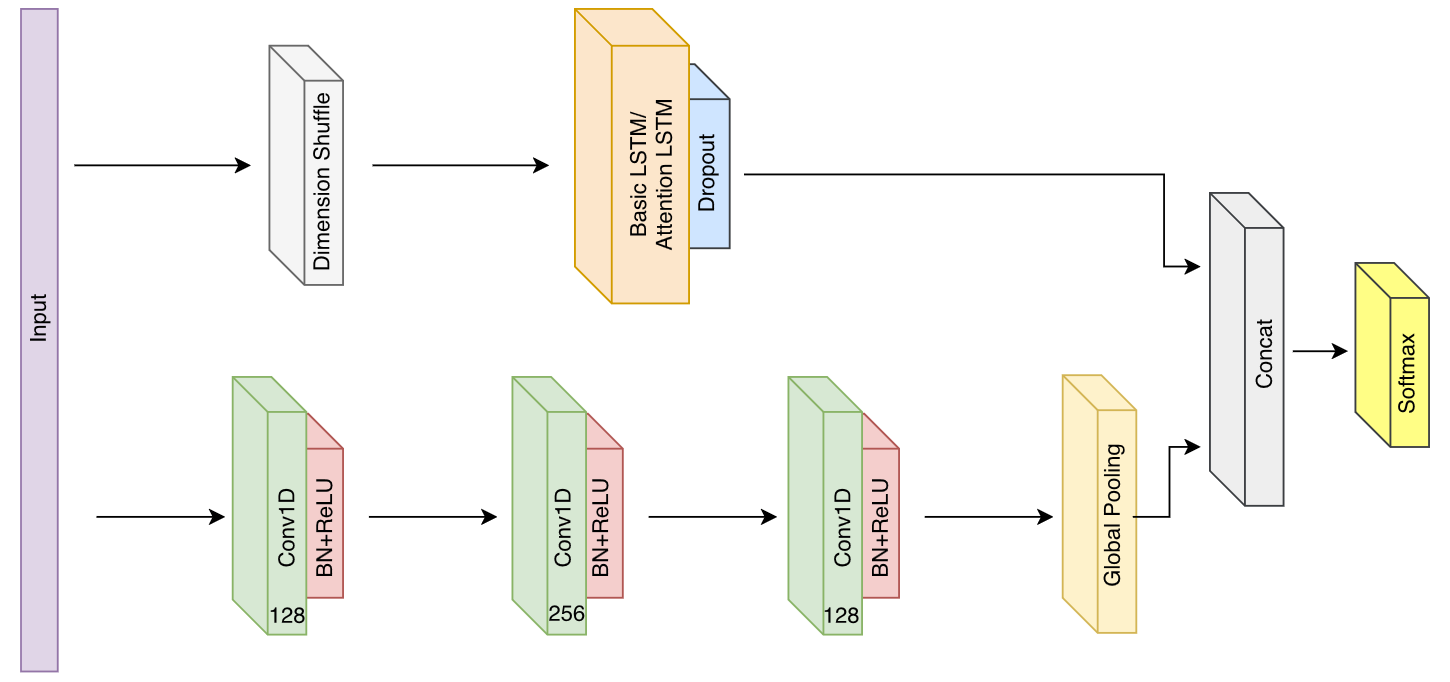
\includegraphics[width=0.75\linewidth]{dissertation//figures/lstm-fcn.png}
    \caption{Architecture for LSTM-FCN\cite{karim2017lstm}}
\end{figure}

\begin{figure}
    \centering
    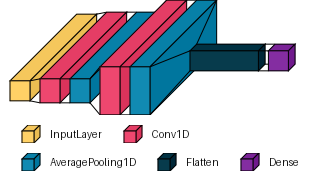
\includegraphics[width=0.5\linewidth]{dissertation//figures/timecnn.png}
    \caption{Architecture of Time-CNN}
\end{figure}

\begin{figure}
    \centering
    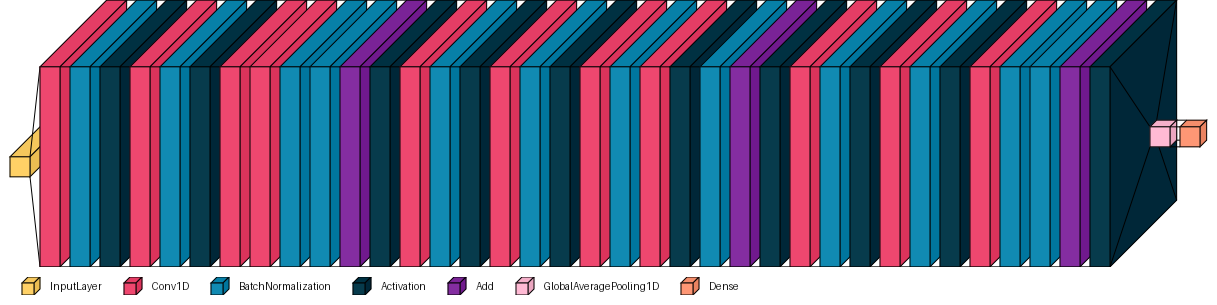
\includegraphics[width=1\linewidth]{dissertation//figures/resnet.png}
    \caption{Architecture of ResNet}
\end{figure}

\begin{figure}
    \centering
    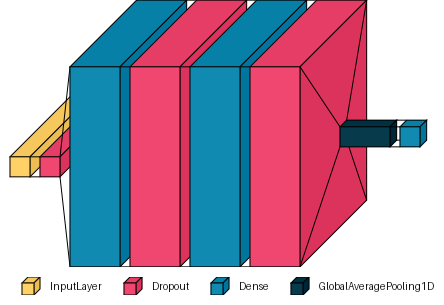
\includegraphics[width=0.5\linewidth]{mlp.png}
    \caption{Architecture of Multi-Layer Perceptron}
\end{figure}

\begin{figure}
    \centering
    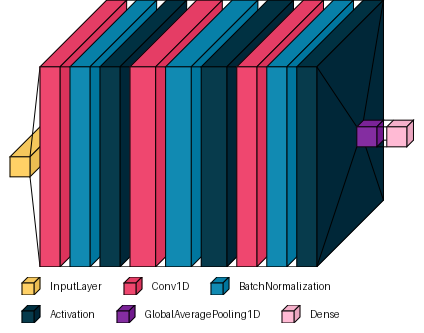
\includegraphics[width=0.5\linewidth]{fcnn.png}
    \caption{Architecture of Fully Convolutional Neural Network}
\end{figure}

\chapter{Traditional Classification Architectures}
\label{ch:trad-architectures}

\begin{figure}[H]
    \centering
    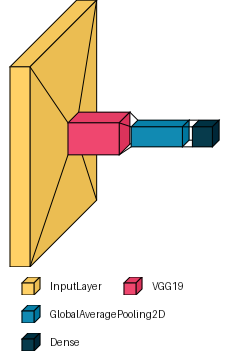
\includegraphics[width=0.4\linewidth]{dissertation//figures/vgg19.png}
    \caption{Architecture of VGG19}
\end{figure}

\begin{figure}[H]
    \centering
    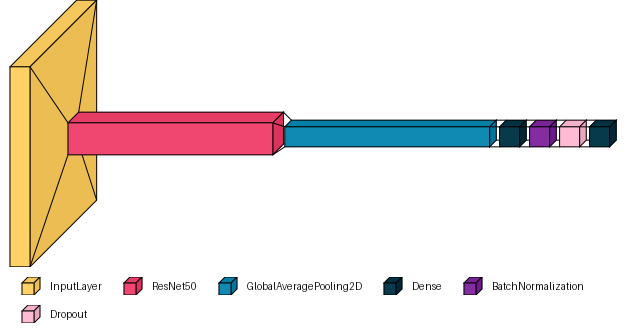
\includegraphics[width=1\linewidth]{dissertation//figures/resnet50.png}
    \caption{Architecture of ResNet}
\end{figure}

\begin{figure}[H]
    \centering
    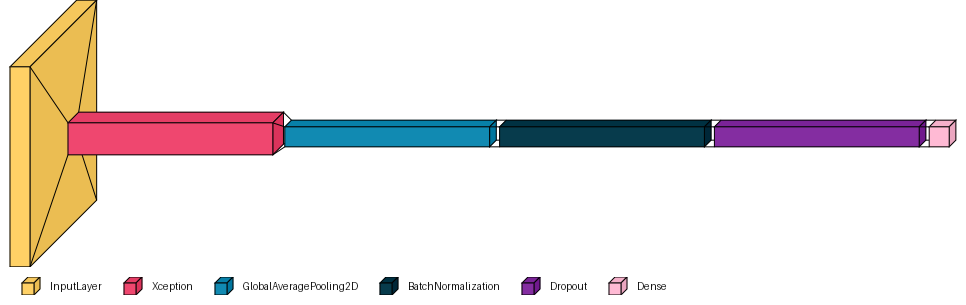
\includegraphics[width=1\linewidth]{dissertation//figures/xception.png}
    \caption{Architecture of Xception}
\end{figure}

\begin{figure}[H]
    \centering
    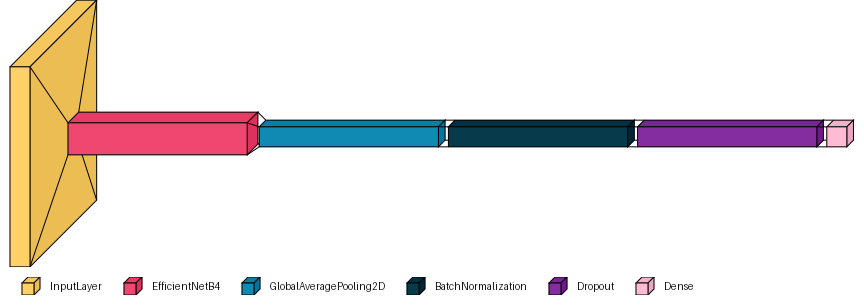
\includegraphics[width=1\linewidth]{dissertation//figures/efficientnet.png}
    \caption{Architecture of EfficientNetB4}
\end{figure}

\chapter{Deep Fake Detection Challenge Website}
\label{ch:dfdcai}

\begin{figure}[h]
    \centering
    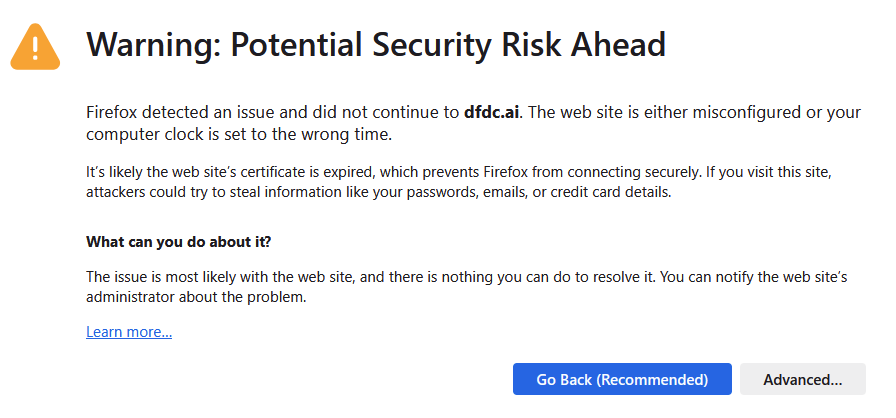
\includegraphics[width=1\linewidth]{dissertation//figures/dfdc.png}
    \caption{A screenshot of the security warning found when trying to access \url{https://dfdc.ai/}}
    \label{fig:dfdcai}
\end{figure}

\chapter{Raw results}
\label{ch:raw-results}

True Positives: declared real when real\\
True Negatives: declared fake when fake\\
False Positives: declared real when fake\\
False Negatives: declared fake when real

\section{Proof of Concept}

\begin{table}[h]
    \centering
    \begin{tabular}{| c | c | c | c | c | c | c |}
        \hline
        \multirow{2}{*}{} & \multicolumn{3}{c|}{\textbf{Unperturbed}} & \multicolumn{3}{c|}{\textbf{Perturbed (VGG, $\epsilon=0.1$)}} \\
        \cline{2-7}
        & \textbf{Blink Detection} & \textbf{VGG} & \textbf{ResNet} & \textbf{Blink Detection} & \textbf{VGG} & \textbf{ResNet} \\
        \hline
        True Positives & 44 & 48 & 45 & 44 & 48 & 45 \\
        \hline
        True Negatives & 36 & 50 & 46 & 32 & 0 & 50 \\
        \hline
        False Positives & 14 & 0 & 4 & 18 & 50 & 0 \\
        \hline
        False Negatives & 6 & 2 & 5 & 6 & 2 & 5 \\
        \hline
        Overall Accuracy & 80\% & 98\% & 91\% & 76\% & 45\% & 95\% \\
        \hline
        Real Accuracy & 88\% & 96\% & 90\% & 88\% & 96\% & 90\% \\
        \hline
        Fake Accuracy & 72\% & 100\% & 92\% & 64\% & 0\% & 100\% \\
        \hline
    \end{tabular}
    \caption{Results of the proof of concept}
    \label{tab:proof-of-concept}
\end{table}

For unperturbed videos, 1 real video and 27 fake videos were classed as unknown. For perturbed videos, 1 real and 18 fake videos were classed as unknown.  

\section{Main Code}

\subsection{FaceForensics}

The time series analysis paired with HRNet was the time series forest.\\
The time series analysis paired with PFLD was learning shapelets.

\begin{table}[H]
    \centering
    \begin{tabular}{|c|c|c|c|c|c|c|}
        \hline
        \textbf{} & \textbf{HRNet} & \textbf{PFLD} &  \textbf{VGG} & \textbf{ResNet} & \textbf{Xception} & \textbf{EfficientNet} \\
        \hline
        True Positives & 113 & 146 & 175 & 182 & 184 & 176\\
        \hline
        True Negatives & 1672 & 2007 & 2813 & 3035 & 2725 & 2889\\
        \hline
        False Positives & 1528 & 1193 & 387 & 165 & 475 & 311\\
        \hline
        False Negatives & 87 & 54 & 25 & 18 & 16 & 24\\
        \hline
        Overall Accuracy & 52.5\% & 63.3\% & 87.9\% & 94.6\% & 85.6\% & 90.1\% \\
        \hline
        Real Accuracy & 56.5\% & 73\% & 87.5\% & 91\% & 92\% & 88\% \\
        \hline
        Fake Accuracy & 52.3\% & 62.7\% & 87.9\% & 94.8\% & 85.2\% & 90.3\% \\
        \hline
    \end{tabular}
    \caption{FaceForensics results unperturbed}
    \label{tab:ff-un}
\end{table}

\begin{table}[H]
    \centering
    \begin{tabular}{|c|c|c|c|c|c|c|}
        \hline
        \textbf{} & \textbf{HRNet} & \textbf{PFLD} &  \textbf{VGG} & \textbf{ResNet} & \textbf{Xception} & \textbf{EfficientNet} \\
        \hline
        True Negatives & 1683 & 2006 & 9 & 486 & 541 & 1069\\
        \hline
        False Positives & 1517 & 1194 & 3191 & 2714 & 2659 & 2131\\
        \hline
        Accuracy & 52.6\% & 62.7\% & 0.2\% & 15.2\% & 16.9\% & 33.4\% \\
        \hline
    \end{tabular}
    \caption{FaceForensics results perturbed (VGG, $\epsilon=0.05$)}
    \label{tab:ff-vgg-5}
\end{table}

\begin{table}[H]
    \centering
    \begin{tabular}{|c|c|c|c|c|c|c|}
        \hline
        \textbf{} & \textbf{HRNet} & \textbf{PFLD} &  \textbf{VGG} & \textbf{ResNet} & \textbf{Xception} & \textbf{EfficientNet} \\
        \hline
        True Negatives & 1730 & 2006 & 0 & 155 & 1086 & 1972\\
        \hline
        False Positives & 1470 & 1194 & 3200 & 3045 & 2114 & 1228\\
        \hline
        Accuracy & 54.1\% & 62.7\% & 0\% & 4.8\% & 33.9\% & 61.6\% \\
        \hline
    \end{tabular}
    \caption{FaceForensics results perturbed (VGG, $\epsilon = 0.1$)}
    \label{tab:ff-vgg-1}
\end{table}

\begin{table}[H]
    \centering
    \begin{tabular}{|c|c|c|c|c|c|c|}
        \hline
        \textbf{} & \textbf{HRNet} & \textbf{PFLD} &  \textbf{VGG} & \textbf{ResNet} & \textbf{Xception} & \textbf{EfficientNet} \\
        \hline
        True Negatives & 1671 & 2005 & 605 & 0 & 507 & 992\\
        \hline
        False Positives & 1529 & 1195 & 2595 & 3200 & 2693 & 2208\\
        \hline
        Accuracy & 52.2\% & 62.7\% & 18.9\% & 0\% & 15.6\% & 31\% \\
        \hline
    \end{tabular}
    \caption{FaceForensics results perturbed (ResNet, $\epsilon=0.05$)}
    \label{tab:ff-res-5}
\end{table}

\begin{table}[H]
    \centering
    \begin{tabular}{|c|c|c|c|c|c|c|}
        \hline
        \textbf{} & \textbf{HRNet} & \textbf{PFLD} &  \textbf{VGG} & \textbf{ResNet} & \textbf{Xception} & \textbf{EfficientNet} \\
        \hline
        True Negatives & 1716 & 2007 & 33 & 0 & 1107 & 1966\\
        \hline
        False Positives & 1484 & 1993 & 3167 & 3200 & 2093 & 1234\\
        \hline
        Accuracy & 53.6\% & 62.7\% & 1\% & 0\% & 34.6\% & 61.4\% \\
        \hline
    \end{tabular}
    \caption{FaceForensics results perturbed (ResNet, $\epsilon=0.1$)}
    \label{tab:ff-res-1}
\end{table}

\begin{table}[H]
    \centering
    \begin{tabular}{|c|c|c|c|c|c|c|}
        \hline
        \textbf{} & \textbf{HRNet} & \textbf{PFLD} &  \textbf{VGG} & \textbf{ResNet} & \textbf{Xception} & \textbf{EfficientNet} \\
        \hline
        True Negatives & 1681 & 2007 & 497 & 267 & 2 & 924\\
        \hline
        False Positives & 1519 & 1193 & 2703 & 2933 & 3198 & 2276\\
        \hline
        Accuracy & 52.5\% & 62.7\% & 15.5\% & 8.3\% & 0\% & 28.9\% \\
        \hline
    \end{tabular}
    \caption{FaceForensics results perturbed (Xception, $\epsilon=0.05$)}
    \label{tab:ff-xce-5}
\end{table}

\begin{table}[H]
    \centering
    \begin{tabular}{|c|c|c|c|c|c|c|}
        \hline
        \textbf{} & \textbf{HRNet} & \textbf{PFLD} &  \textbf{VGG} & \textbf{ResNet} & \textbf{Xception} & \textbf{EfficientNet} \\
        \hline
        True Negatives & 1699 & 2007 & 27 & 178 & 1 & 1921\\
        \hline
        False Positives & 1501 & 1193 & 3173 & 3022 & 3199 & 1279 \\
        \hline
        Accuracy & 53.1\% & 62.6\% & 0.1\% & 5.6\% & 0\% & 60\% \\
        \hline
    \end{tabular}
    \caption{FaceForensics results perturbed (Xception, $\epsilon=0.1$)}
    \label{tab:ff-xce-1}
\end{table}

\begin{table}[H]
    \centering
    \begin{tabular}{|c|c|c|c|c|c|c|}
        \hline
        \textbf{} & \textbf{HRNet} & \textbf{PFLD} &  \textbf{VGG} & \textbf{ResNet} & \textbf{Xception} & \textbf{EfficientNet} \\
        \hline
        True Negatives & 1673 & 2006 & 605 & 425 & 537 & 0\\
        \hline
        False Positives & 1527 & 1194 & 2595 & 2775 & 2663 & 3200\\
        \hline
        Accuracy & 52.3\% & 62.7\% & 18.9\% & 13.3\% & 16.8\% & 0\% \\
        \hline
    \end{tabular}
    \caption{FaceForensics results perturbed (EfficientNet, $\epsilon=0.05$)}
    \label{tab:ff-eff-5}
\end{table}

\begin{table}[H]
    \centering
    \begin{tabular}{|c|c|c|c|c|c|c|}
        \hline
        \textbf{} & \textbf{HRNet} & \textbf{PFLD} &  \textbf{VGG} & \textbf{ResNet} & \textbf{Xception} & \textbf{EfficientNet} \\
        \hline
        True Negatives & 1722 & 2008 & 33 & 134 & 1085 & 0\\
        \hline
        False Positives & 1478 & 1992 & 3167 & 3066 & 2115 & 3200\\
        \hline
        Accuracy & 53.8\% & 62.8\% & 1\% & 4.2\% & 33.9\% & 0\% \\
        \hline
    \end{tabular}
    \caption{FaceForensics results perturbed (EfficientNet, $\epsilon=0.1$)}
    \label{tab:ff-eff-1}
\end{table}

\subsection{Celeb-DF}

The time series analysis paired with HRNet was learning shapelets.\\
The time series analysis paired with PFLD was learning shapelets.

\begin{table}[H]
    \centering
    \begin{tabular}{|c|c|c|c|c|c|c|}
        \hline
        \textbf{} & \textbf{HRNet} & \textbf{PFLD} &  \textbf{VGG} & \textbf{ResNet} & \textbf{Xception} & \textbf{EfficientNet} \\
        \hline
        True Positives & 103 & 104 & 165 & 174 & 172 & 171\\
        \hline
        True Negatives & 3021 & 2930 & 4838 & 4896 & 4833 & 4877\\
        \hline
        False Positives & 1906 & 1997 & 89 & 31 & 94 & 50\\
        \hline
        False Negatives & 75 & 74 & 13 & 4 & 6 & 7\\
        \hline
        Overall Accuracy & 61.2\% & 59.4\% & 98\% & 99.3\% & 98\% & 98.9\% \\
        \hline
        Real Accuracy & 57.9\% & 58.4\% & 92.7\% & 97.8\% & 96.6\% & 96.1\% \\
        \hline
        Fake Accuracy & 61.3\% & 59.5\% & 98.2\% & 99.4\% & 98.1\% & 99\% \\
        \hline
    \end{tabular}
    \caption{Celeb-DF results unperturbed}
    \label{tab:cd-un}
\end{table}

\begin{table}[H]
    \centering
    \begin{tabular}{|c|c|c|c|c|c|c|}
        \hline
        \textbf{} & \textbf{HRNet} & \textbf{PFLD} &  \textbf{VGG} & \textbf{ResNet} & \textbf{Xception} & \textbf{EfficientNet} \\
        \hline
        True Negatives & 3020 & 2937 & 0 & 4040 & 4647 & 486\\
        \hline
        False Positives & 1907 & 1990 & 4927 & 887 & 280 & 4441\\
        \hline
        Accuracy & 61.3\% & 59.6\% & 0\% & 82\% & 94.3\% & 9.9\% \\
        \hline
    \end{tabular}
    \caption{Celeb-DF results perturbed (VGG, $\epsilon=0.05$)}
    \label{tab:cd-vgg-5}
\end{table}

\begin{table}[H]
    \centering
    \begin{tabular}{|c|c|c|c|c|c|c|}
        \hline
        \textbf{} & \textbf{HRNet} & \textbf{PFLD} &  \textbf{VGG} & \textbf{ResNet} & \textbf{Xception} & \textbf{EfficientNet} \\
        \hline
        True Negatives & 3021 & 2952 & 0 & 4927 & 3754 & 4\\
        \hline
        False Positives & 1906 & 1957 & 4927 & 0 & 1173 & 4923\\
        \hline
        Accuracy & 61.3\% & 59.9\% & 0\% & 100\% & 76.2\% & 0.1\% \\
        \hline
    \end{tabular}
    \caption{Celeb-DF results perturbed (VGG, $\epsilon = 0.1$)}
    \label{tab:cd-vgg-1}
\end{table}

\begin{table}[H]
    \centering
    \begin{tabular}{|c|c|c|c|c|c|c|}
        \hline
        \textbf{} & \textbf{HRNet} & \textbf{PFLD} &  \textbf{VGG} & \textbf{ResNet} & \textbf{Xception} & \textbf{EfficientNet} \\
        \hline
        True Negatives & 3019 & 2939 & 215 & 0 & 4582 & 414\\
        \hline
        False Positives & 1908 & 1988 & 4712 & 4927 & 345 & 4513\\
        \hline
        Accuracy & 61.3\% & 59.7\% & 4.3\% & 0\% & 93\% & 8.4\% \\
        \hline
    \end{tabular}
    \caption{Celeb-DF results perturbed (ResNet, $\epsilon=0.05$)}
    \label{tab:cd-res-5}
\end{table}

\begin{table}[H]
    \centering
    \begin{tabular}{|c|c|c|c|c|c|c|}
        \hline
        \textbf{} & \textbf{HRNet} & \textbf{PFLD} &  \textbf{VGG} & \textbf{ResNet} & \textbf{Xception} & \textbf{EfficientNet} \\
        \hline
        True Negatives & 3021 & 2952 & 103 & 3357 & 3724 & 3\\
        \hline
        False Positives & 1906 & 1975 & 4824 & 1570 & 1203 & 4924\\
        \hline
        Accuracy & 61.3\% & 59.9\% & 2.1\% & 68.1\% & 75.6\% & 0.1\% \\
        \hline
    \end{tabular}
    \caption{Celeb-DF results perturbed (ResNet, $\epsilon=0.1$)}
    \label{tab:cd-res-1}
\end{table}

\begin{table}[H]
    \centering
    \begin{tabular}{|c|c|c|c|c|c|c|}
        \hline
        \textbf{} & \textbf{HRNet} & \textbf{PFLD} &  \textbf{VGG} & \textbf{ResNet} & \textbf{Xception} & \textbf{EfficientNet} \\
        \hline
        True Negatives & 3020 & 2936 & 193 & 3323 & 2 & 134\\
        \hline
        False Positives & 1907 & 1991 & 4734 & 1604 & 4925 & 4793\\
        \hline
        Accuracy & 61.3\% & 59.6\% & 3.9\% & 67.4\% & 0\% & 2.7\% \\
        \hline
    \end{tabular}
    \caption{Celeb-DF results perturbed (Xception, $\epsilon=0.05$)}
    \label{tab:cd-xce-5}
\end{table}

\begin{table}[H]
    \centering
    \begin{tabular}{|c|c|c|c|c|c|c|}
        \hline
        \textbf{} & \textbf{HRNet} & \textbf{PFLD} &  \textbf{VGG} & \textbf{ResNet} & \textbf{Xception} & \textbf{EfficientNet} \\
        \hline
        True Negatives & 3021 & 2951 & 96 & 4927 & 0 & 3\\
        \hline
        False Positives & 1906 & 1976 & 4831 & 0 & 4927 & 4924\\
        \hline
        Accuracy & 61.3\% & 59.9\% & 1.9\% & 100\% & 0\% & 0\% \\
        \hline
    \end{tabular}
    \caption{Celeb-DF results perturbed (Xception, $\epsilon=0.1$)}
    \label{tab:cd-xce-1}
\end{table}

\begin{table}[H]
    \centering
    \begin{tabular}{|c|c|c|c|c|c|c|}
        \hline
        \textbf{} & \textbf{HRNet} & \textbf{PFLD} &  \textbf{VGG} & \textbf{ResNet} & \textbf{Xception} & \textbf{EfficientNet} \\
        \hline
        True Negatives & 3019 & 2938 & 215 & 3955 & 4580 & 0\\
        \hline
        False Positives & 1908 & 1988 & 4712 & 972 & 347 & 4927\\
        \hline
        Accuracy & 61.3\% & 59.6\% & 4.4\% & 80.3\% & 93\% & 0\% \\
        \hline
    \end{tabular}
    \caption{Celeb-DF results perturbed (EfficientNet, $\epsilon=0.05$)}
    \label{tab:cd-eff-5}
\end{table}

\begin{table}[H]
    \centering
    \begin{tabular}{|c|c|c|c|c|c|c|}
        \hline
        \textbf{} & \textbf{HRNet} & \textbf{PFLD} &  \textbf{VGG} & \textbf{ResNet} & \textbf{Xception} & \textbf{EfficientNet} \\
        \hline
        True Negatives & 3021 & 2952 & 96 & 4927 & 0 & 3\\
        \hline
        False Positives & 1906 & 1975 & 4831 & 0 & 4927 & 4924\\
        \hline
        Accuracy & 61.3\% & 59.9\% & 1.9\% & 100\% & 0\% & 0\% \\
        \hline
    \end{tabular}
    \caption{Celeb-DF results perturbed (EfficientNet, $\epsilon=0.1$)}
    \label{tab:cd-eff-1}
\end{table}

\section{Transferability}
\label{sec:transfer}

\begin{table}[H]
    \centering
    \begin{tabular}{|c|c|c|c|c|c|c|}
        \hline
        \textbf{} & \textbf{HRNet} & \textbf{PFLD} & \textbf{VGG} & \textbf{ResNet} & \textbf{Xception} & \textbf{EfficientNet} \\
        \hline
        True Positives & 345 & 119 & 485 & 492 & 494 & 482\\
        \hline
        True Negatives & 2512 & 6414 & 4269 & 1500 & 2332 & 2956\\
        \hline
        False Positives & 7197 & 3295 & 5440 & 8209 & 7377 & 8209\\
        \hline
        False Negatives & 155 & 381 & 15 & 8 & 6 & 18\\
        \hline
        Overall Accuracy & 28\% & 64\% & 46.6\% & 19.5\% & 27.7\% & 33.7\% \\
        \hline
        Real Accuracy & 69\% & 23.8\% & 97\% & 98.4\% & 98.8\% & 96.4\% \\
        \hline
        Fake Accuracy & 25.9\% & 66.1\% & 44\% & 15.4\% & 24\% & 30\% \\
        \hline
    \end{tabular}
    \caption{The accuracy of models trained on FaceForensics and tested on FakeAVCeleb}
\end{table}

\begin{table}[H]
    \centering
    \begin{tabular}{|c|c|c|c|c|c|c|}
        \hline
        \textbf{} & \textbf{HRNet} & \textbf{PFLD} & \textbf{VGG} & \textbf{ResNet} & \textbf{Xception} & \textbf{EfficientNet} \\
        \hline
        True Positives & 3 & 148 & 500 & 500 & 500 & 499\\
        \hline
        True Negatives & 9678 & 5699 & 344 & 427 & 317 & 657\\
        \hline
        False Positives & 31 & 4010 & 9365 & 9282 & 9392 & 9052\\
        \hline
        False Negatives & 397 & 352 & 0 & 0 & 0 & 1\\
        \hline
        Overall Accuracy & 94.8\% & 57.3\% & 8.3\% & 9.1\% & 8\% & 11.3\% \\
        \hline
        Real Accuracy & 0.6\% & 29.6\% & 100\% & 100\% & 100\% & 99.8\% \\
        \hline
        Fake Accuracy & 99.7\% & 58.7\% & 3.5\% & 4.4\% & 3.3\% & 6.8\% \\
        \hline
    \end{tabular}
    \caption{The accuracy of models trained on Celeb-DF and tested on FakeAVCeleb}
\end{table}

\chapter{Open Source Contributions}
\label{ch:open-source}

\url{https://github.com/bethgelab/foolbox/pull/738}

\begin{figure}[h]
    \centering
    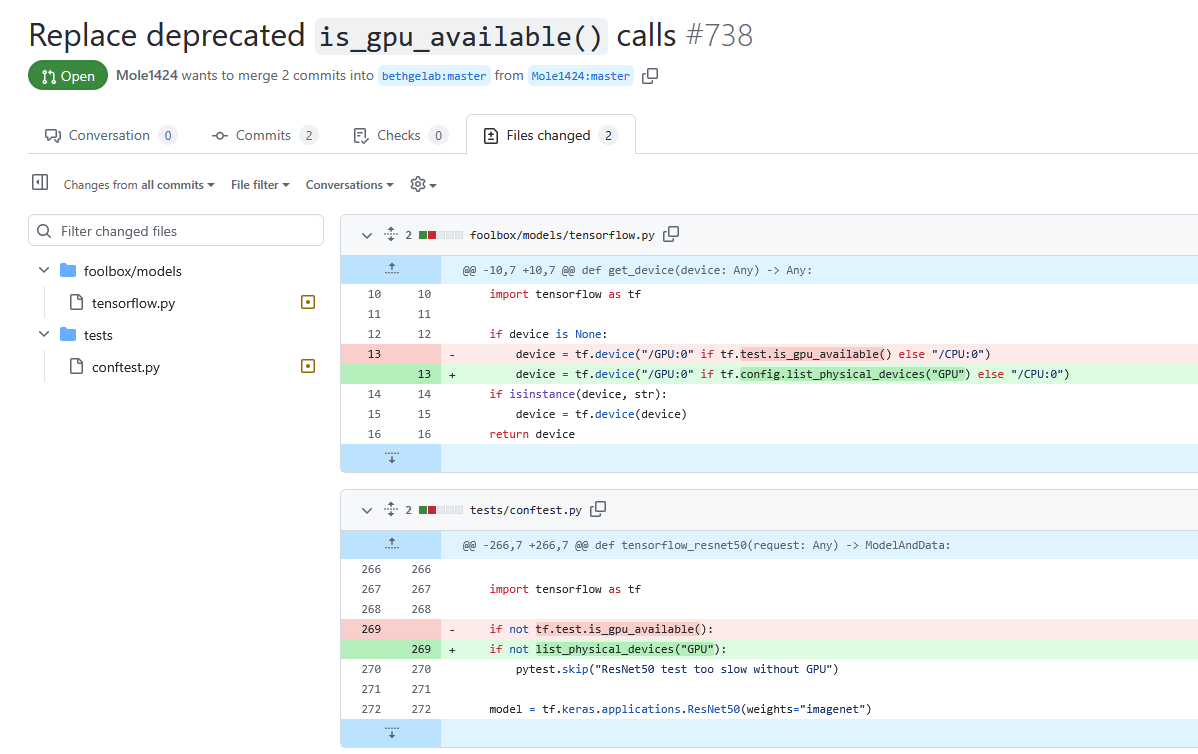
\includegraphics[width=\linewidth]{dissertation//figures/pull-request.png}
    \caption{A pull request made to the FoolBox\cite{rauber2017foolbox}\cite{rauber2017foolboxnative} library to replace a deprecated TensorFlow function}
\end{figure}

\url{https://gist.github.com/Jsevillamol/0daac5a6001843942f91f2a3daea27a7}

\begin{figure}[h]
    \centering
    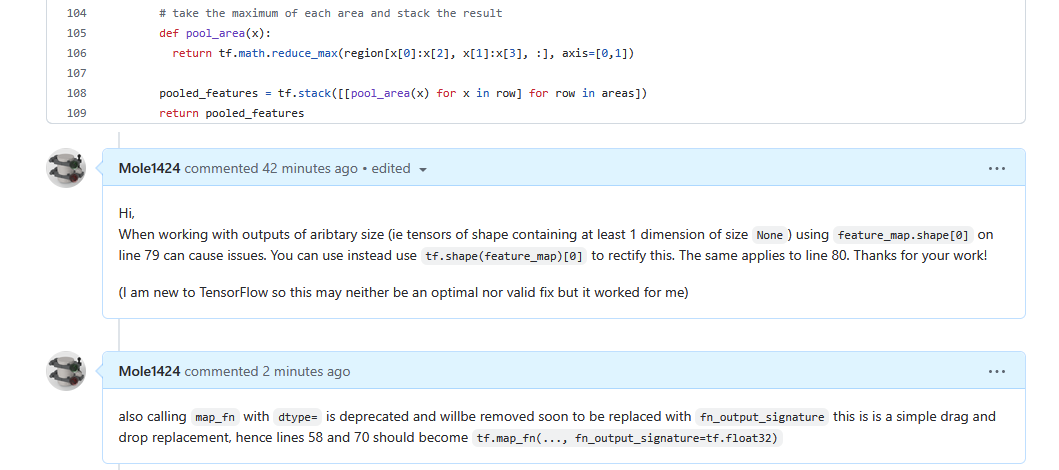
\includegraphics[width=1\linewidth]{dissertation//figures/comment.png}
    \caption{A comment made to an ROI pooling implementation to allow for variable sizing in images}
\end{figure}